\documentclass{ctexart}
\usepackage{amsmath, mathrsfs, amsfonts}
\usepackage{tikz}
\usepackage{graphicx}
% library



\begin{document}
\begin{figure}[htp]
    \centering
    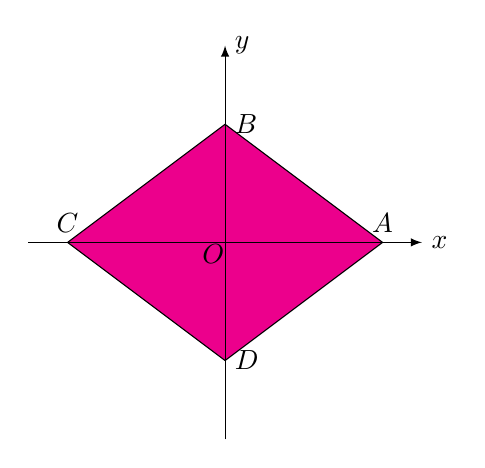
\begin{tikzpicture}[>=latex,scale=.5]
        \draw[fill=magenta] (-4,0)node[above]{$C$}--(0,3)node[right]{$B$}--(4,0)node[above]{$A$}--(0,-3)
        node[right]{$D$}--(-4,0);

        \draw[->] (-5,0)--(5,0)node[right]{$x$};
        \draw[->] (0,-5)--(0,5)node[right]{$y$};
        \node at (-.3,-.3){$O$};

    \end{tikzpicture}

    \caption{<caption>}
\end{figure}

\begin{figure}[htp]
    \centering
    
\begin{tikzpicture}[>=latex]
        % \draw[fill=cyan] (0,0) rectangle (4,3);    % 存在边框
        % \fill [cyan] (0,0) rectangle (4,3);    % 没有边框
        \fill [cyan, draw=black] (0,0) rectangle (4,3);    % 跟第一个效果一样


    \end{tikzpicture}

    \caption{<caption>}
\end{figure}

\begin{figure}[htp]
    \centering
    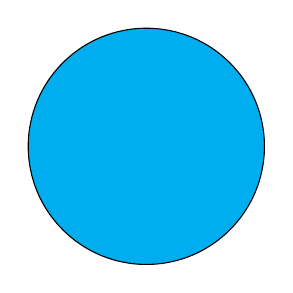
\begin{tikzpicture}[>=latex]
        \draw[fill=cyan] (0,0) circle (1.5);


    \end{tikzpicture}

    \caption{<caption>}
\end{figure}

\begin{figure}[htp]
    \centering
    \begin{tikzpicture}[>=latex]
        \draw (0,0)--(4,0);
        % \draw (0,0)--(4,4);
        \draw (0,0)--(45:4);    % 以极坐标的方式进行画图

        \draw[->] (2,0) arc (0:45:2);    % 圆弧的绘制



    \end{tikzpicture}

    \caption{<caption>}
\end{figure}







\end{document}